
\section{Helical Antenna}
\subsection{要求}
\noindent 
根据轴向模螺旋天线驻波(普通端射模式)的方向图计算公式
\begin{equation}
E=\sin\left(\frac{\pi}{2N}\right)\cos\theta\dfrac{\sin\left[\left(N/2\right)\psi\right]}{\sin\left[\psi/2\right]}.
\end{equation}
其中
\begin{equation}
\psi=k_0\left(S\cos\theta-\frac{L_0}{p}\right), p=\frac{L_0/\lambda_0}{S/\lambda_0 +1}.
\end{equation}
画出一个沿z轴放置、$N=8$圈、螺距$S=\lambda/4$、单圈线长$L_0=\lambda$的轴向模螺旋天线的竖直平面(x=0)方向图。

\noindent 选做:

1.根据天线的对称性,利用编程数据计算$D_0$,并与经验公式$D_0\simeq15n\dfrac{c^2S}{\lambda_0^3}$
的结果进行比较


\subsection{原理及推导}
分析方向图计算公式发现$E\sim\left(N,S,L,\theta\right)$. 在编程的时候输入参量$S,L$均是以$\lambda$为单位, 所以$\psi$可以化简如下
\begin{equation}
\psi=2\pi\left(S\cos\theta-\frac{L}{p}\right), p=\frac{L}{S+1}.
\end{equation}
故编程时写作
\begin{lstlisting}[language={matlab},keywordstyle=\color{blue!70},commentstyle=\color{red!50!green!50!blue!50},frame=shadowbox, rulesepcolor=\color{red!20!green!20!blue!20}] 
p=L/(S+1);
psi=2*pi*(S*cos(theta)-L/p);
A=sin(pi/2/N);
B=cos(theta);
C=sin(N/2*psi)./sin(psi/2);
E=A.*B.*C;
Power=E.^2;
\end{lstlisting}

计算方向性的经验公式, 约去$\lambda_0$后, 得到
\begin{equation}
D=15Nc^2 S
\end{equation}
\subsection{结果与分析}
\subsubsection{方向图及$D_0$}
归一化,非dB的辐射功率方向图如图\ref{fig:HelixP}所示, 为了观察后瓣情况, 放大图如图\ref{fig:HelixP_fangda}. 
\begin{figure}[!ht]
	%\small
	\centering
	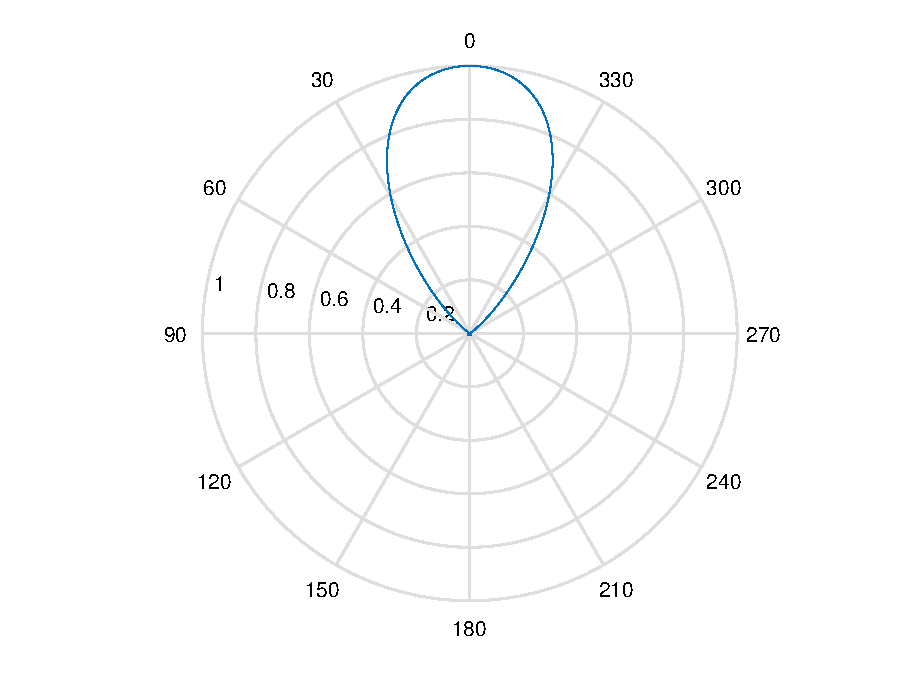
\includegraphics[width=10cm]{HelixPattern.eps}
	\caption{Helical Antenna Pattern} \label{fig:HelixP}
\end{figure}

\begin{figure}[!ht]
	%\small
	\centering
	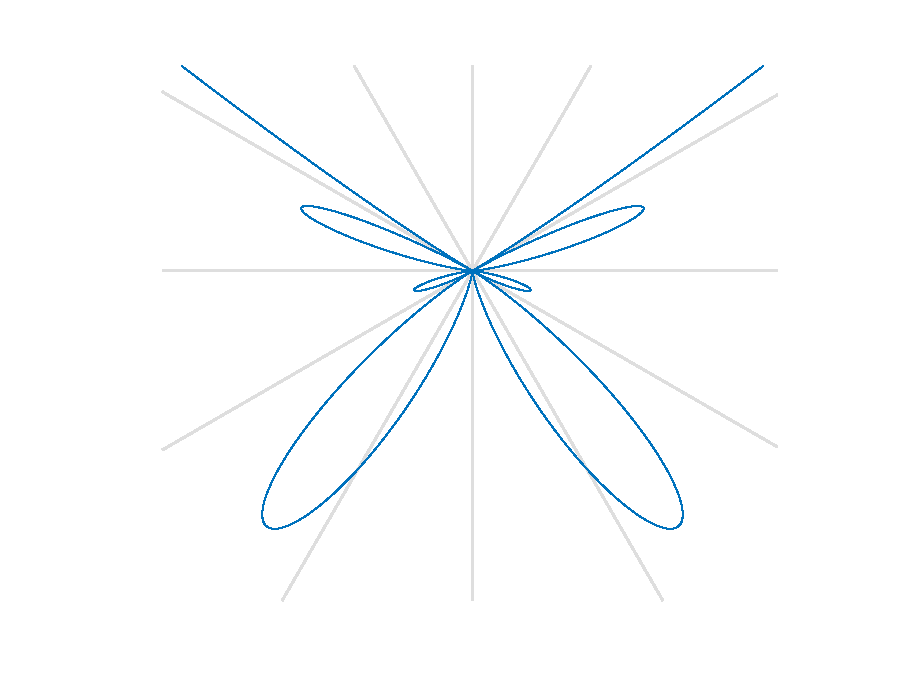
\includegraphics[width=10cm]{HelixPattern_fangda.eps}
	\caption{放大图} \label{fig:HelixP_fangda}
\end{figure}




\subsubsection{选做:与经验公式的对比}
经验公式计算结果为:
\begin{equation}
D=15Nc^2 S=15N(L^2-S^2) S=28.125.
\end{equation}
所以$D=14.49\,dB$.


编程计算的结果为$D_0=12.40\,dB$与经验公式相比,是在接受范围之内的. 
\newpage
\subsection{程序}
\noindent \textbf{主程序}
\begin{lstlisting}[language={matlab},keywordstyle=\color{blue!70},commentstyle=\color{red!50!green!50!blue!50},frame=shadowbox, rulesepcolor=\color{red!20!green!20!blue!20}] 
clear
close all
N=8;S=0.25;L=1;
Fun_Helix(N,S,L)
%Compare equation
clear
syms theta
N=8;S=0.25;L=1;
p=L/(S+1);
psi=2*pi*(S*cos(theta)-L/p);
A=sin(pi/2/N);
B=cos(theta);
C=sin(N/2*psi)/sin(psi/2);
E=A*B*C;
Power=E^2;
PP=cos(theta)*sin(8*pi*(0.25*cos(theta)-1.25))/sin(pi*(0.25*cos(theta)-1.225));
a=vpa(int(2*pi*Power,theta,[0,2*pi]),6)
D=10*log10(a)
% b=int(PP,theta,[0,2*pi])
% vpa(b,6)
% D=4*pi*2.4359/a;

D_exp=10*log10(15*N*(L^2-S^2)*S)



\end{lstlisting}
\noindent \textbf{子函数}
\begin{lstlisting}[language={matlab},keywordstyle=\color{blue!70},commentstyle=\color{red!50!green!50!blue!50},frame=shadowbox, rulesepcolor=\color{red!20!green!20!blue!20}] 
function Fun_Helix(N,S,L)
%Polar Pattern
%Input N,S/Lambda,L0/lambda
%Output D is directivity
theta=linspace(0,2*pi,5000);
p=L/(S+1);
psi=2*pi*(S*cos(theta)-L/p);
A=sin(pi/2/N);
B=cos(theta);
C=sin(N/2*psi)./sin(psi/2);

E=A.*B.*C;
Power=E.^2;
polar(theta,Power/max(Power));
view(-90,90)
% max(E.^2)
% D=max(Power)/mean(Power);
end
\end{lstlisting}